\documentclass[a4paper,12pt]{article}

% Any percent sign marks a comment to the end of the line

% Every latex document starts with a documentclass declaration like this
% The option dvips allows for graphics, 12pt is the font size, and article
%   is the style

\usepackage[pdftex]{graphicx}
%\usepackage{url}
\usepackage{hyperref}
% These are additional packages for "pdflatex", graphics, and to include
% hyperlinks inside a document.
\usepackage{lettrine}
\setlength{\oddsidemargin}{0.25in}
%\setlength{\textwidth}{6.5in}
\setlength{\topmargin}{0in}
%\setlength{\textheight}{8.5in}

% These force using more of the margins that is the default style
\usepackage{times}
\usepackage{mathptmx}
\usepackage{color}
\usepackage{amssymb}
\usepackage{amsmath}
\begin{document}

% Everything after this becomes content
% Replace the text between curly brackets with your own

\title{Final Report: Epic-Monopoly}
\author{\small Ziqiang Li\quad Yulian Mao\quad Xizi Ni\quad Yilin Zheng\quad Chenyu Zhou\\
\small \{11510352, 11510086, 11510602, 11510506, 11510374\}@mail.sustc.edu.cn}
\date{\today}

% You can leave out "date" and it will be added automatically for today
% You can change the "\today" date to any text you like


\maketitle

% This command causes the title to be created in the document

\section{Abstract}
\lettrine[lines=2,loversize=0.35,lraise=0.07,findent=3pt,nindent=2pt]{I}{}n this project, we concentrate on developing a new web-based monopoly game mechanism which called Epic-Monopoly. We do this since the original monopoly game is rigid in rules and less exciting for players after some turns. There are many new and interesting element evolved in this game. Economy factor, similar to GDP or relative index, is added into the game as an approach to model the reality. The index of assets value, tax rate and punishment intensity of chance cards are all under the influence of this mechanism. For more user flexibility, the difficulty of the game can be adjusted at the very beginning of a game by changing initial cash and some other indexes. In the course of a game, we use dynamic map aiming to make a more interesting but still balanceable experience. The player falling behind might catch up again with this change. In the reality, there are many cooperation between entrepreneurs that might influence tax and warfare, so, this game includes alliance and countries which can also be seen as loyalty program to model this situation. Despite of those important and creative new silver point, there are some other modification, such as the enterprisers mid entering rules. The details are introduced in the following sections. Besides, we will give more details of the requirements the program involved, concrete implementation and UI design of the game as well as the future work we plan to do. 
\section{Motivation}
\lettrine[lines=2,loversize=0.35,lraise=0.07,findent=3pt,nindent=2pt]{T}{}he program comes from the SCORE 2018 contest and is also a course project for our OOP course. We choose this project since   designing and making a game from zero to one is something exciting. Besides, the game we design, is an old but popular game since $1989$ and we all have ever played and known the boring experience with the rigid rules without any interesting challenges and changes. So, to create something new based on its origin is a good idea and we will also learn much about game design and object oriented programming if we applies the technique we picked up from OOP course. This is the rough motivation which contributes to our choice on this idea and making efforts on this project.
\section{User Benefits}
\lettrine[lines=2,loversize=0.35,lraise=0.07,findent=3pt,nindent=2pt]{T}{}his is a novel game compared with original monopoly game. We add many new features and mechanisms which can make the course of the game more fancy and attractive. We do not expect   any money return since it will finally becomes an open source project on GitHub but we hope that more people can get happiness by playing our games and give us constructive advice or support. Future benefits can be discussed but so far we cannot expected too much.

\section{Requirements \& Features}	\lettrine[lines=2,loversize=0.35,lraise=0.07,findent=3pt,nindent=2pt]{T}{}his project is a web-based game design project so it involves web development techniques and the requirements of this production includes all the fundamental features and some new features the sponsor wants:
\begin{itemize}
	\item allow players to enable a random sequence of spots as well as a periodic, random change of the properties pricing, rents, interests and taxes rates (in both spots and cards);
	\item allow a loyalty program to enable the use of virtual currency with random rules based on existing international alliances’ programs;
	\item allow new players to join the game as entrepreneurs (weaker restrictions on the number of players);
	\item allow complexity setting in three levels (e.g., easy, medium, hard) based on rules and different configurations from exploring variabilities on the previous three bullets.
\end{itemize}

To meet these requirements, we add some new features as following:
 
\begin{itemize}
	\item Economy Factor
	
	Analogy from GDP or some relative economic index, Economy Factor(EF) is considered in the Epic-Monopoly. EF act as a “global ruler”, is in charge of the change of the price of properties, tax and value of other object. Also, introducing EF in to Epic-Monopoly can also balance the game dynamically.
	
	For a specific period, EF will change between a certain range, and it will have influence on the rent, pricing of the house, etc. Because of its characteristic, the average value of all property is same. It is seldom for a property devalue every period, which is unfortunate for the owner of this property.
	
	\item Dynamic Map
	The sequence of spot in the Epic-Monopoly will change in a specific period, to repick the fate of players who falling behind. To unified the map, the change of color blocks, stations and utilities will be control by some rules.
	
	\item Country \& Alliance
	
	For the cooperation problem, countries and alliances are introduced to the Epic-Monopoly. Every player will assign to one countries and corresponding alliances. The trade and rent between the member of alliances will make discount. And some new event will add to opportunity, to add more fun. In reality, tax and warfare differ depends of country’s policy. Therefore, the tax and some of cards in society chest will depends on which country the player belongs.
	
	\item Difficulty Setting
	
	Players can custom some game configuration, to simplified this process, difficult setting is introduced to the Epic-Monopoly. The difficulty most depends on the fluctuation of the game parameter. For example, easy model the EF setting will within $5\%$ while normal model will be $10\%$. 
	
	\item Adding enterpriser during the game
	
	Enterprisers are allowed to join the game after the game began. However, the enterprisers only able to join when unman real estate more than $50\%$. And the initial cash of the enterprisers is depended on how many turn the game have begun.
	
	\item Loyalty Program
	
	Instead of return cash or virtual currency, Epic-Monopoly will make discount for enterpriser. (The effect is same, but simpler) With the time enterpriser enter other’s spot, the rent of the spot to this enterpriser will decrease.  Same rules for prison. With the time an enterpriser bail from the prison, the price will increase, which is similar to reality (The more in to prison, the more bail fee it has to paid).
\end{itemize}	


\section{Design principle}
\begin{itemize}
	\item Object Oriented\\  
    Epic-Monopoly is designed by object-oriented ideas. At the begining, it took us over one week to design the UML which further helped us a lot during the implementation. The main game logic is divided into several parts and every part is defined by some super classes. For example, the "Block" class is the super class which represents all the block in the chess board. The "Block" can be further divided to "Asset" which represents the properties in the game, "CardPile" which represents the "Chance" and "Chest" block in the chess board. And those sub-classes can be divided into even smaller class, "Asset" can be divided into "Estate", "Utility" and "Station", which are the three main properties that players owns in during the game. Every sub-class have their own game logic and attributes but share many same attributes like "name", "id" and "position". The benifits of using object-oriented design, on the one hand can reduce the lines of code, on the other hand, let us focus more on the difference between classes. Also, it is very convenient to debug and further maintain as well. At the end of this project, we found a extremely wired bug. After analysis and tests on it, we realized it happend in the common codes among "Estate", "Utility" and "Station", thus we are able to find the mistake and repair it.
    Moreover, there are many similar methods used in the program. For example, payment, is used by many objects to process a trading case. Therefore, we extract this kind of methods to a file named "operation", and almost all classes will import this module since they need the common method. It will also prevent the re-import problem. We do the same procedure when we designed the "messenger" class again. It embedded all the methods about communication between client and server.
	\item Speed\\
    Epic-Monopoly is a web-based game. User are not willing to wait for several seconds or even minutes for the initializaion of a game. While we loading the files from server, the user can use those time to create a room or join a room. The loading time much tougher to observe. Also, we use CDN to delivering the data quickly, which speeds up the initialization and reduces the pressure of our server.
	\item Safety\\
    The game logic runs only on the server, and both the front and back end will check the details and results of the game, ensuring possibility for players to cheat.
	\item Balancing\\
    There are many feature introduced in the new monopoly, to balance the game and maximize the happiness of players. Epic-Monopoly was tested to balance the new features and original game settings.
\end{itemize}

\section{Implementation}
\lettrine[lines=2,loversize=0.35,lraise=0.07,findent=3pt,nindent=2pt]{I}{}
mplementation includes front end and back end. Here we just roughly state the detail of front end and the communication between front end and back end. Back end is implemented by Python $3.6.4$ and the game logic is described in previous section.


Front end includes \textbf{page design} and \textbf{animation design}. 

For \textbf{page design}:

There are two pages in Epic-Monopoly. The first is login page and the second is game page. 
	
In login page, we use a \textless canvas \textgreater element as a container, a \textless form\textgreater to collect players' personal configuration (nickname and avatar) including an \textless input type="text"\textgreater element and a \textless select\textgreater element. 

Then if player chooses to create a room, a hidden \textless div\textgreater element will be displayed, which contains another \textless form\textgreater. That \textless form\textgreater contains an \textless input type="text"\textgreater element, several groups of \textless input type="radio"\textgreater elements and \textless input type="checkbox"\textgreater element, to set up all configurations of the new room. After player confirming his settings, the function \emph{createRoom} will be called. It then calls \emph{getPlayerJson} and \emph{getRoomJson} to obtain all settings of the player in JSON form and sends a HTTP POST to transfer the aggregated JSON to the server. Then read the JSON returned by the server and stores them in sessionStorage, and finally let the window jump to the game page.

And if player chooses to join a room, the function \emph{getRoomList} will be called. It sends a HTTP GET request to the server to get all information of existing rooms at that time, then reads the JSON returned by the server and adds data into a \textless table\textgreater element in another hidden \textless div\textgreater element, and finally displays the hidden \textless div\textgreater. Then player can join any room that is still not filled by $6$ players. After that function \emph{joinRoom} will be called. It then calls \emph{getPlayerJson} to obtain all settings of the player in JSON form and also the room whom player chose to join and sends a HTTP POST to transfer the aggregated JSON to the server, then read the JSON returned by the server and stores them in sessionStorage, and finally lets the window jump to the game page.
	
The game page is divided into three parts: left part, mid part and right part. The left part contains two \textless div\textgreater elements: one to displays room information, another to display all players and their basic information in the room. Each player is displayed in a \textless div\textgreater elements containing an \textless img\textgreater (to display avatar), two \textless span\textgreater (to display player’s name and cash) and an \textless a\textgreater (as a trade button). The player \textless div\textgreater elements are all hidden and will be displayed when a new player joins the room. 

The mid part contains a \textless button\textgreater to start gaming and a hidden \textless div\textgreater. When player presses the start button and the room is permitted to start a game, the button will be hidden and the hidden \textless div\textgreater containing the chessboard will be displayed. 

The right part contains two \textless div\textgreater, record and states. The record contains an inner \textless div\textgreater to display all record of the game and the states contains a \textless table\textgreater to display some dynamic data during the game.


For \textbf{animation design}:
\begin{itemize}
	\item sessionStorage: store room id, users' id, users' avatar. And these data will be cleaned when the browser closed.
	\item Chessboard part:\\
	Chessboard is a canvas, there are two main parts in chessboard to implement the animation design: \emph{preload} and \emph{create}. We put \emph{update} part into the \emph{create} part since we need JSON data when initializing the chessboard.\\
	We only use \textbf{Phaser} game framework in our project.
	\begin{itemize}
		\item The first part is preload. In this part, we load our elements including images and spritesheets. We also new a \textbf{WebSocket} object here to build communication with back end.
		\item The second part is a function: \emph{WebSocketTest}\\
		We implement the actions according to the JSON files sent by back end
		\begin{itemize}
			\item Init:
			\begin{itemize}
				\item Create the part of chessboard which will not change during the game. Such as the four corners , chest blocks and chance blocks.
				\item Create the rest part of chessboard according to the JSON file, such as estate, station and utility.
				\item Create the players on the "Go" block.
			\end{itemize}
		\item Update:
		\begin{itemize}
			\item Update the block information
			\item Update the players' information including their position, cash 
			\item Update estate, station, utility information
			\item Bank information
			\item Economic Factor
		\end{itemize}
	\item Hint:
	\begin{itemize}
		\item Show message on the screen last two seconds.
	\end{itemize}
		\end{itemize}
		\item  Some isolated functions:
		\begin{itemize}
			\item create\_house: creates houses or hotels according to the house number of the block information
			\item listener \& show\_block\_infoContect: shows the cressponding information window(estate information window, ) when click the block sprite
			\item roll\_dice: control dice rolling action
			\item mortgage: send a mortgage request when click the mortgage button
		\end{itemize}
	\end{itemize}
\end{itemize}

Another import part is the \textbf{communication} between client and server.
Our server is based on Tornado which is a Python web framework and asynchronous networking library. Its two features are what our game program needs. Tornado deals with all requests from client in our present architecture. Server will monitor all room members (clients) if their links are alive. If not, the server will destroy the room, close the socket, empty the memory for the rest of other games. 

The program doesn’t have an account management system, and we consider that a player who creates or joins a room is ready for starting games. We also allow that players join a game which is ongoing, but follow the rules on initial cash for balancing the game.

If room owner creates a room, the server will not create a game immediately. Until the room has enough players and one of them clicked “start game” the server will create a new game instance in another threading. Also, the server threading communicates with the game threading through pipe, which notifies the game threading the clients activities. The game message uses a queue to preventing from blocking on received or sent messages.


\section{User Interface}
\lettrine[lines=2,loversize=0.35,lraise=0.07,findent=3pt,nindent=2pt]{T}{}here are two pages in Epic-Monopoly: \textbf{welcome page} and \textbf{game page}. Each has several sub-interfaces by displaying some hidden elements. 

Some main interfaces are listed as follows. For the detail information, please refer to appendix II.
\begin{itemize}
	\item Welcome Page \\
	Players will see the welcome page firstly when they access to our website. They can set nickname and choose avatar and then start a game by creating a room or joining certain room other players created. 
	\item Waiting Interface\\ 
	After entering a room and before starting a game, players can only see a “start game” button in the center of the window.
 	\item In-game Main Interface\\ 
 	During the game, the chessboard, two dices as well as some operating buttons will be laid in the center of the website page, with players locations and buildings and ownerships of spaces showed in a simple and clear way. Room number, players information and conditions are on the left. Record for all events and dynamic arguments are displayed on the right side. 
	\item Chessboard\\ 
	Our chessboard is developed based on game engine Phaser designed based on the one in classical version. The layout is same as the classical monopoly game. But icons and color schemes are our unique style. 
	\item In-game Check \& Management Interface\\ 
	When click any space on the chessboard, a small table will be shown in the center of the chessboard. It includes information of that space and buttons to operate it (only for the owner). 
	\item In-game Trading Interface\\
	When click any other player on the left, trade interface will come out on the center, where all optional spaces will be listed with check boxes.
\end{itemize}

\section{Future work}
We have some features still need to be fully tested and codes are still need improvement. In future we will refactor our codes and perfect our UI which might takes much time to finish and meet our original expectation.


%uncomment follwoing to use refrence
%\begin{thebibliography}{99}

%\bibitem{gonzalez2012} Jonay I. Gonz\'{a}lez Hern\'{a}ndez, 
%Pilar Ruiz-Lapuente,	
%Hugo M. Tabernero,	
%David Montes,	
%Ramon Canal,	
%Javier M\'{e}ndez	
%and Luigi R. Bedin,
%{No surviving evolved companions of the progenitor of SN1006},
%Nature, {\bf 489}, 533-536 (2012).

%\end{thebibliography}

\section*{Appendix I-UML}

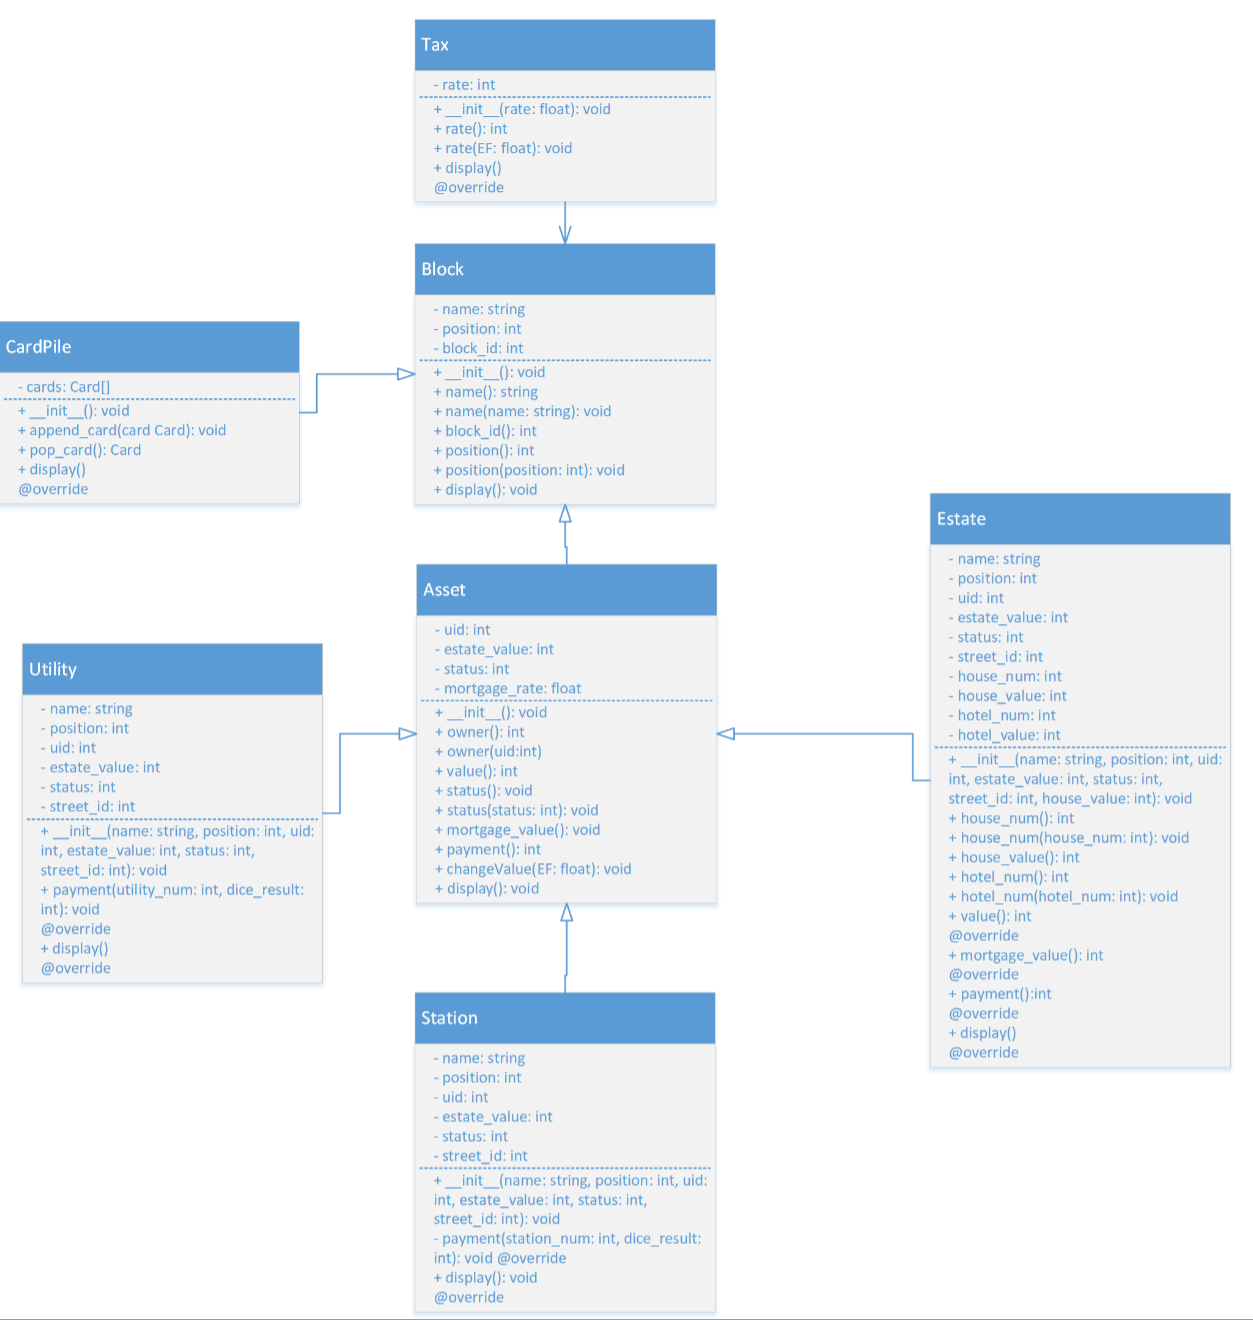
\includegraphics[scale=0.9]{image/Block.png}
\\
\\
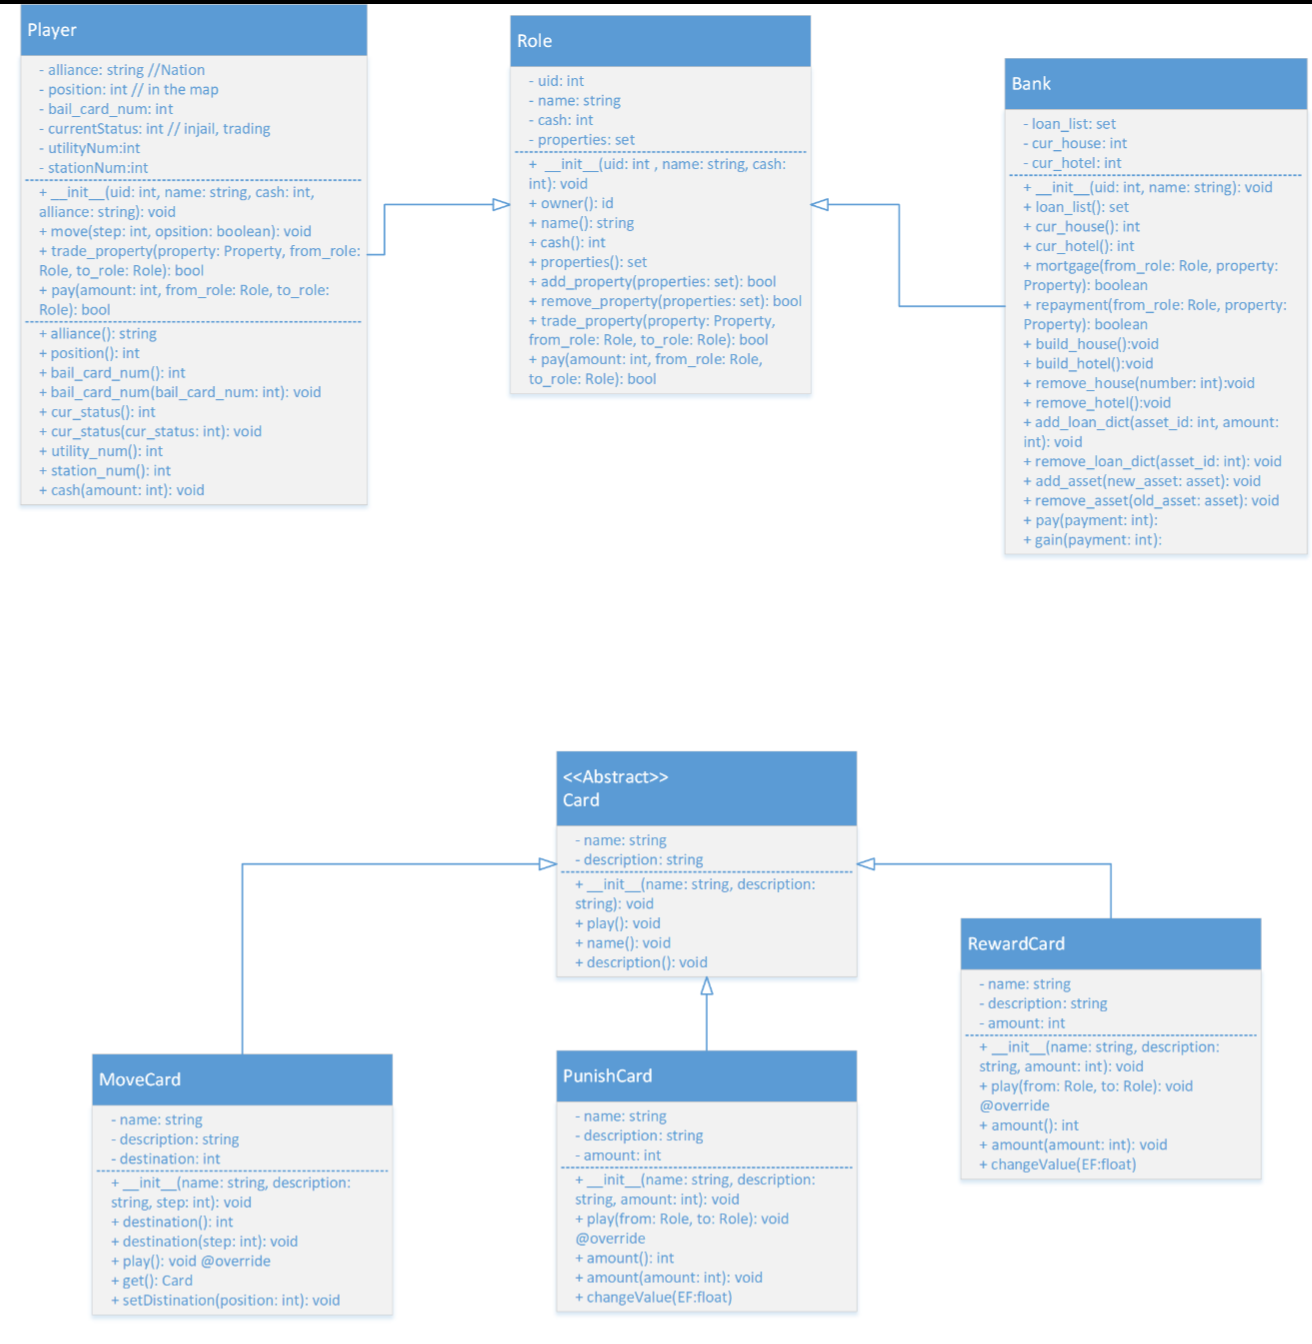
\includegraphics[scale=0.9]{image/roleandcard.png}
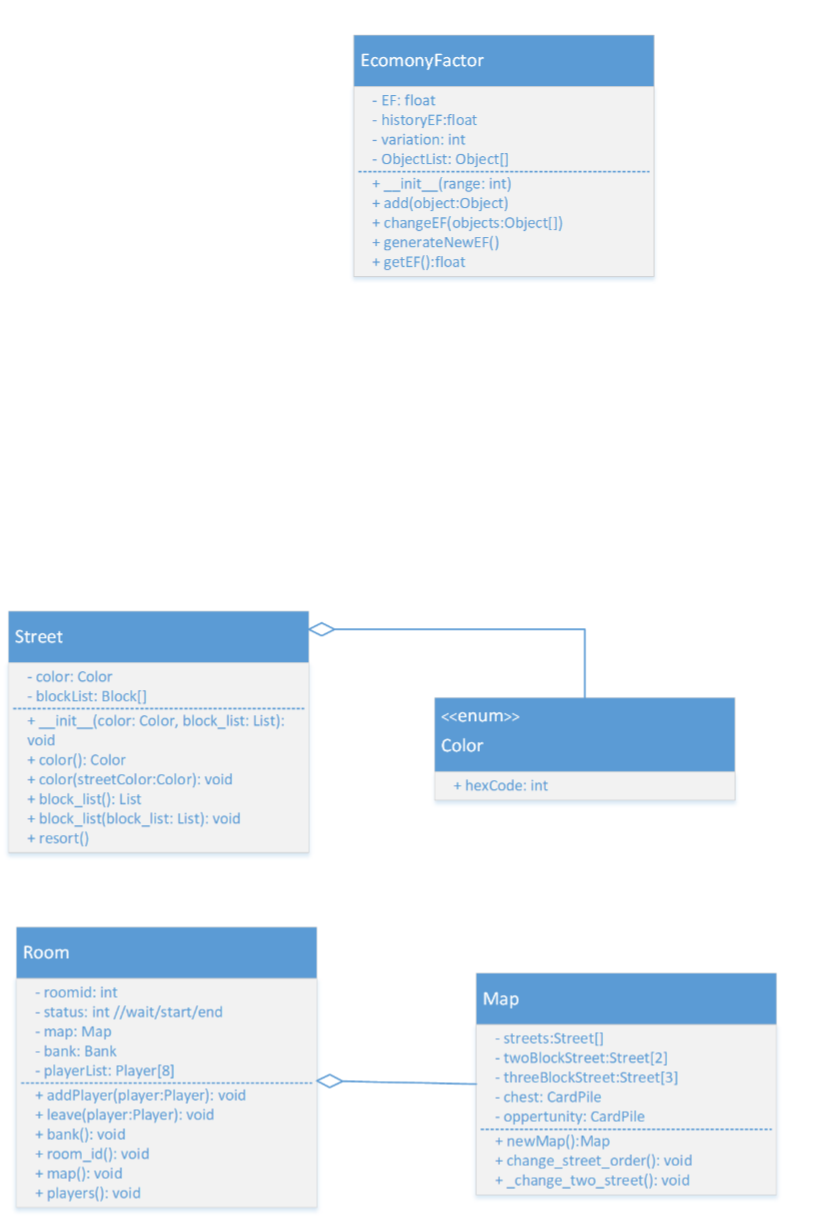
\includegraphics[scale=1.3]{image/efandmain.png}
\section*{Appendix II-UI}
\begin{figure}[htbp]
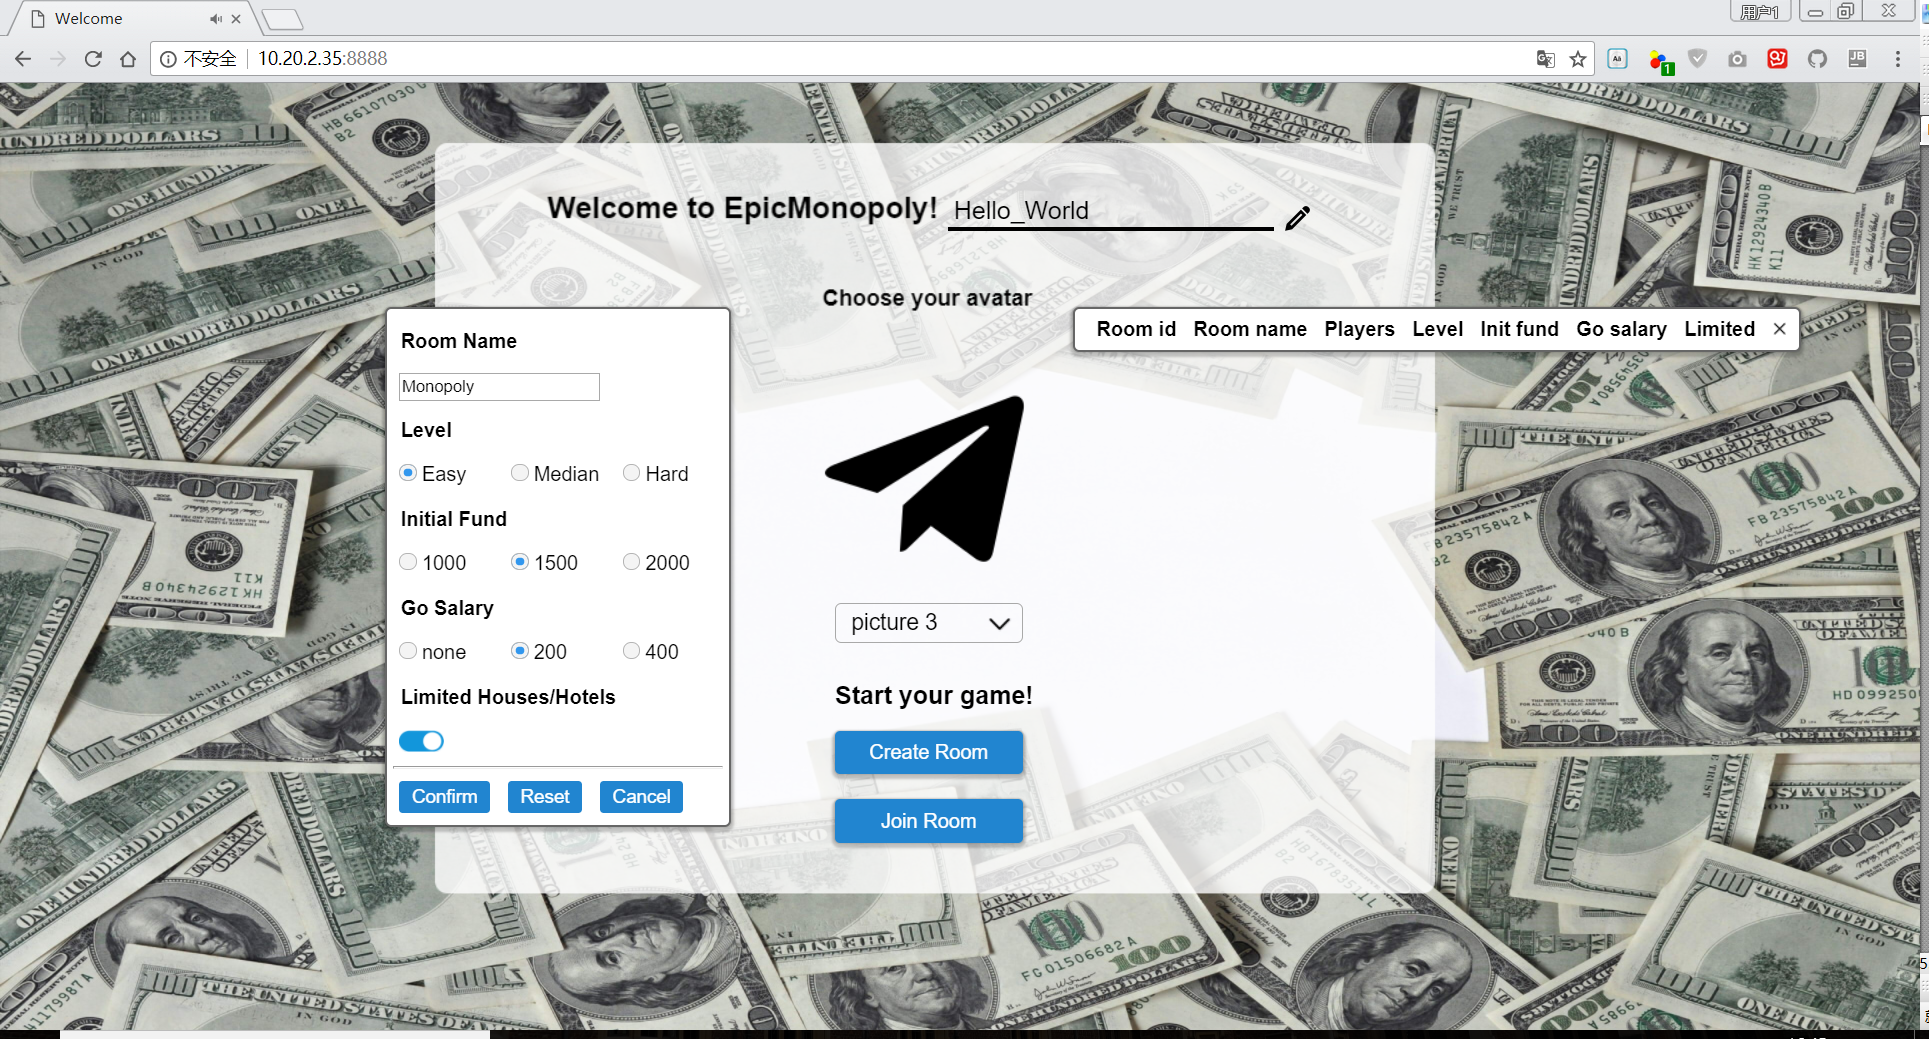
\includegraphics[scale=0.32]{image/login.png}
\caption{Settings}
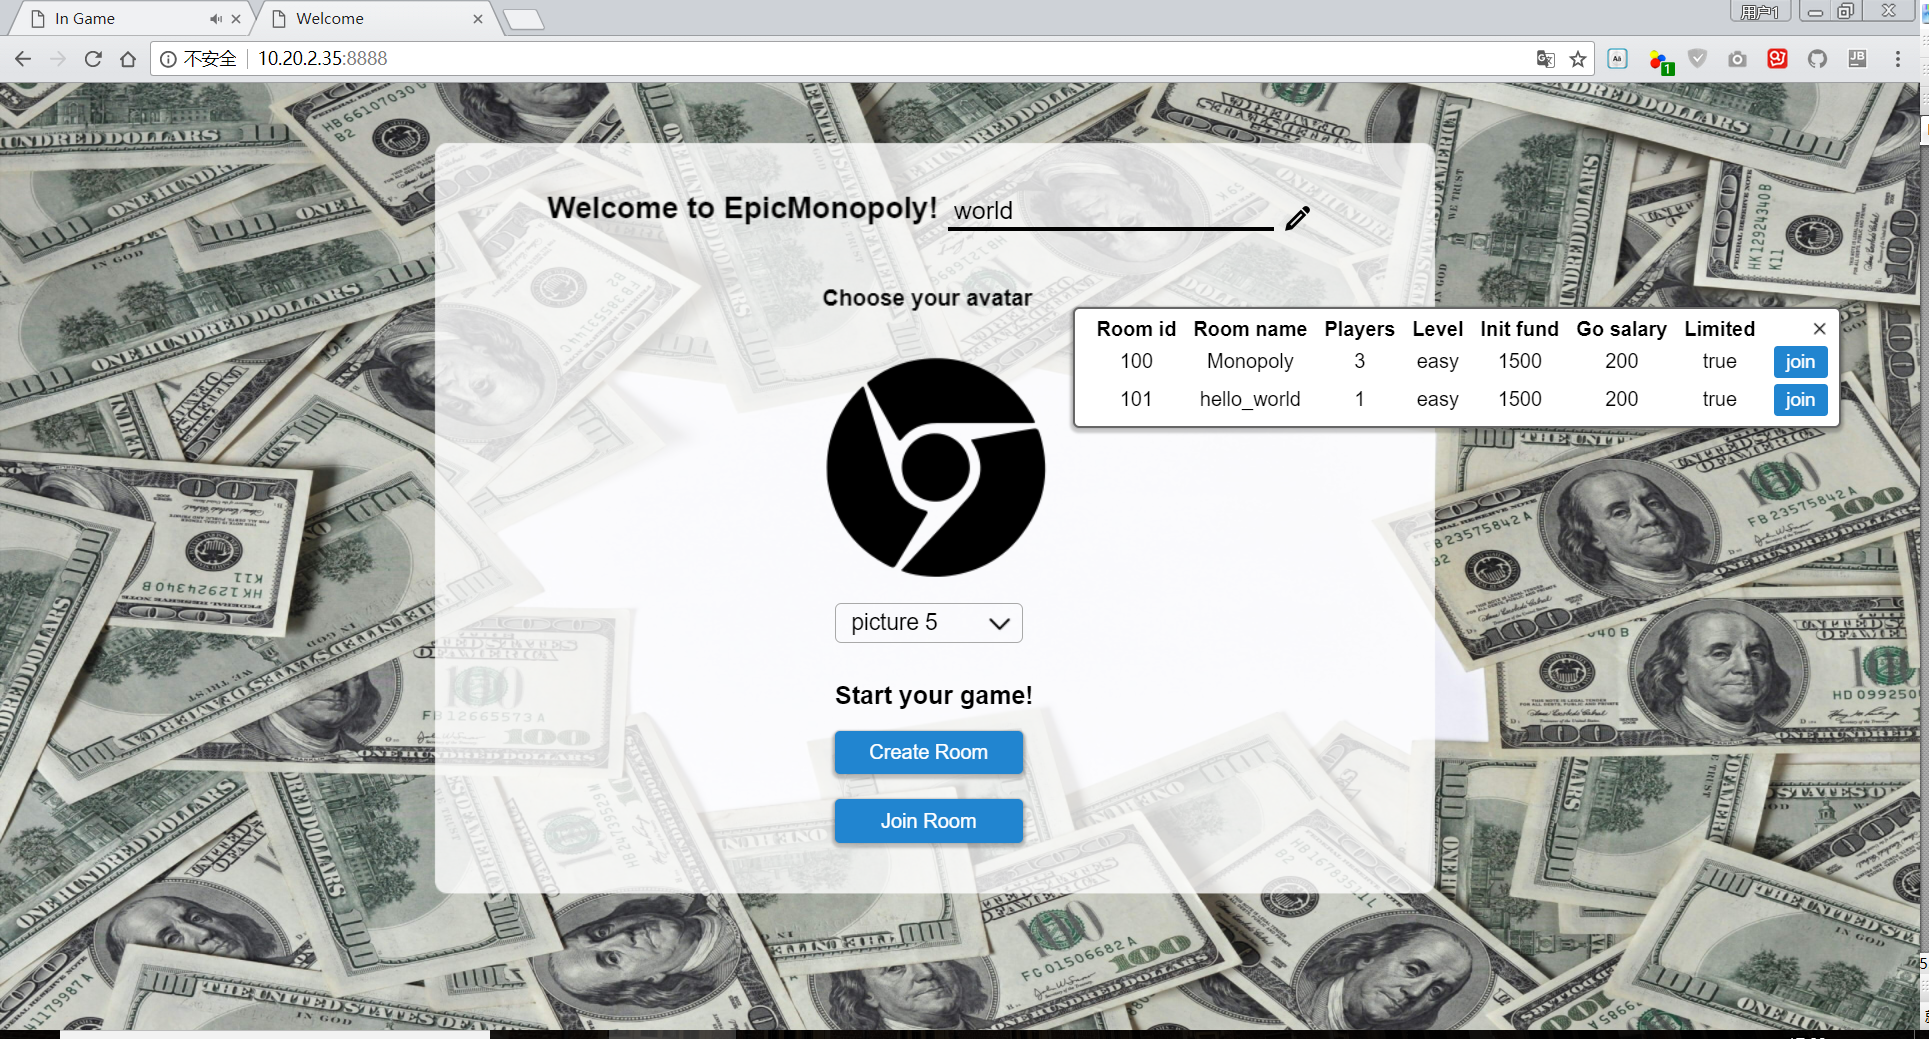
\includegraphics[scale=0.32]{image/login1.png}
\caption{Room List}
\end{figure}
\begin{figure}[htbp]
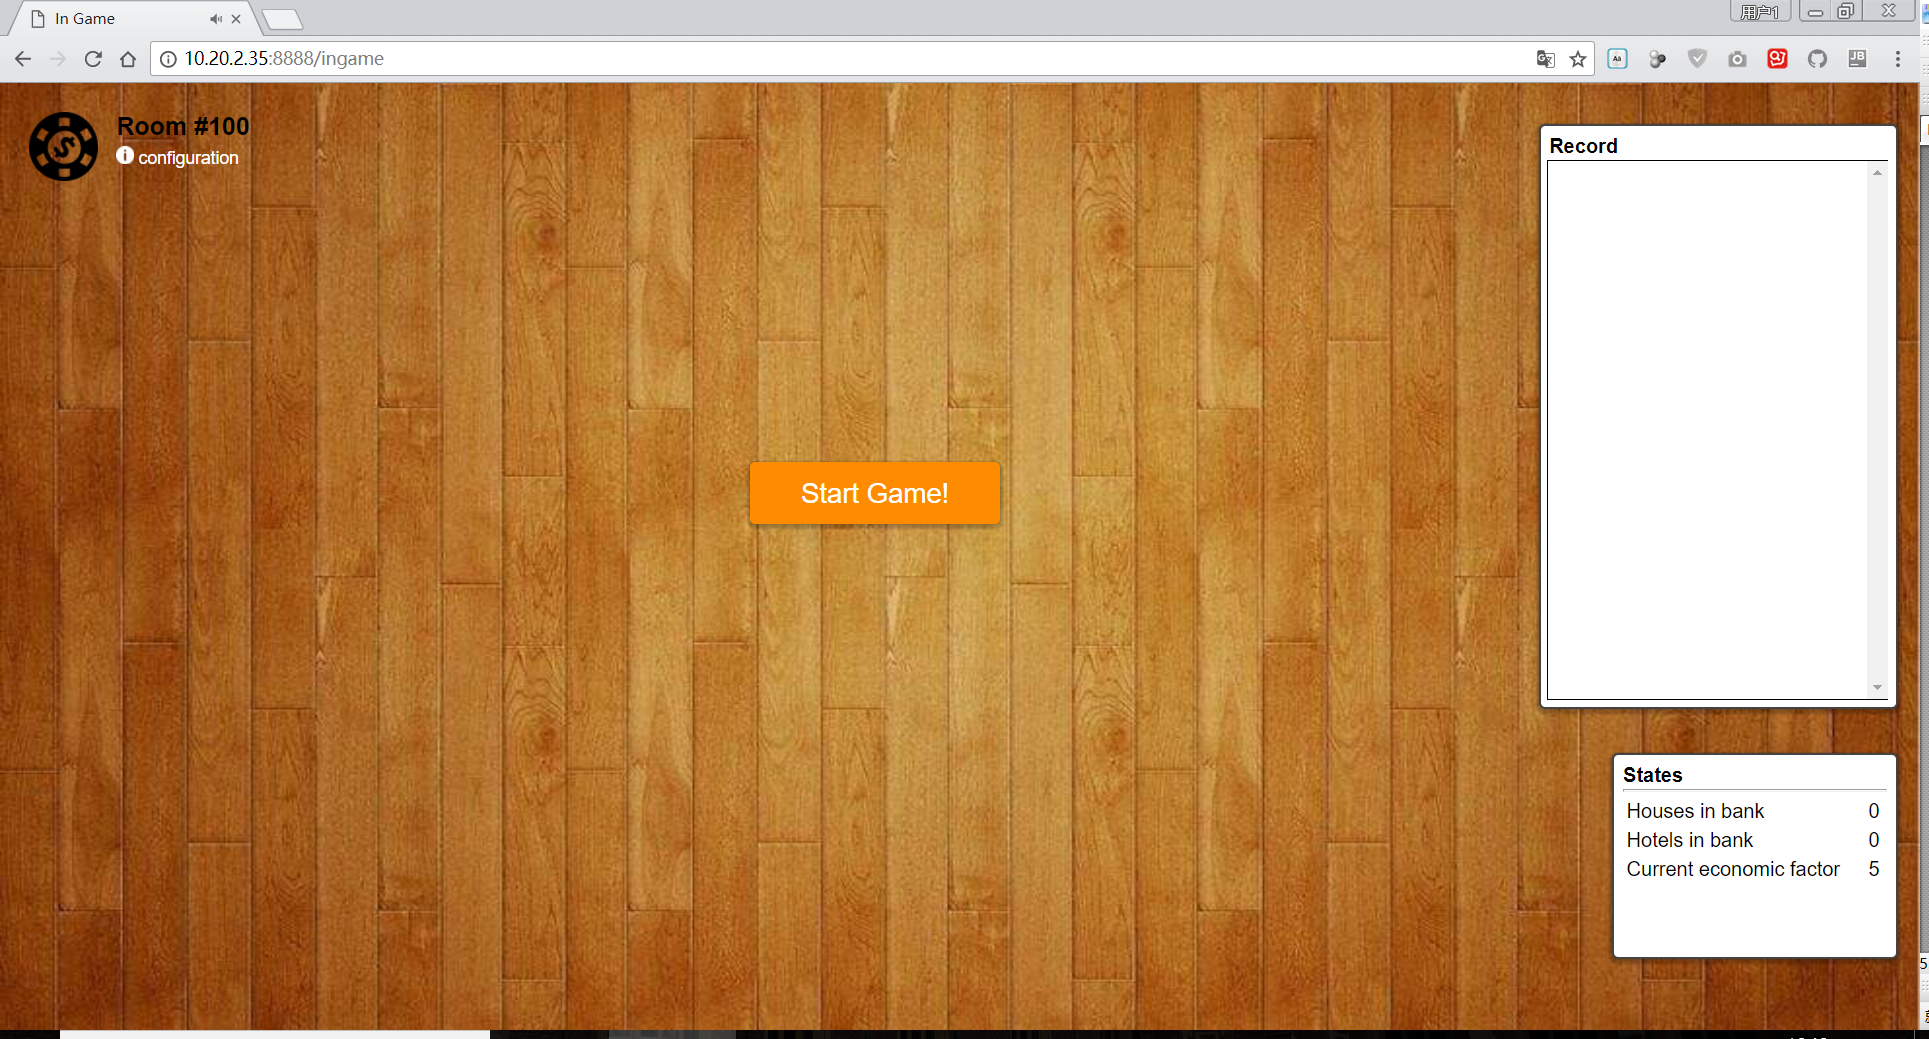
\includegraphics[scale=0.32]{image/start_game.png}
\caption{Start page}
\end{figure}
\begin{figure}[htbp]
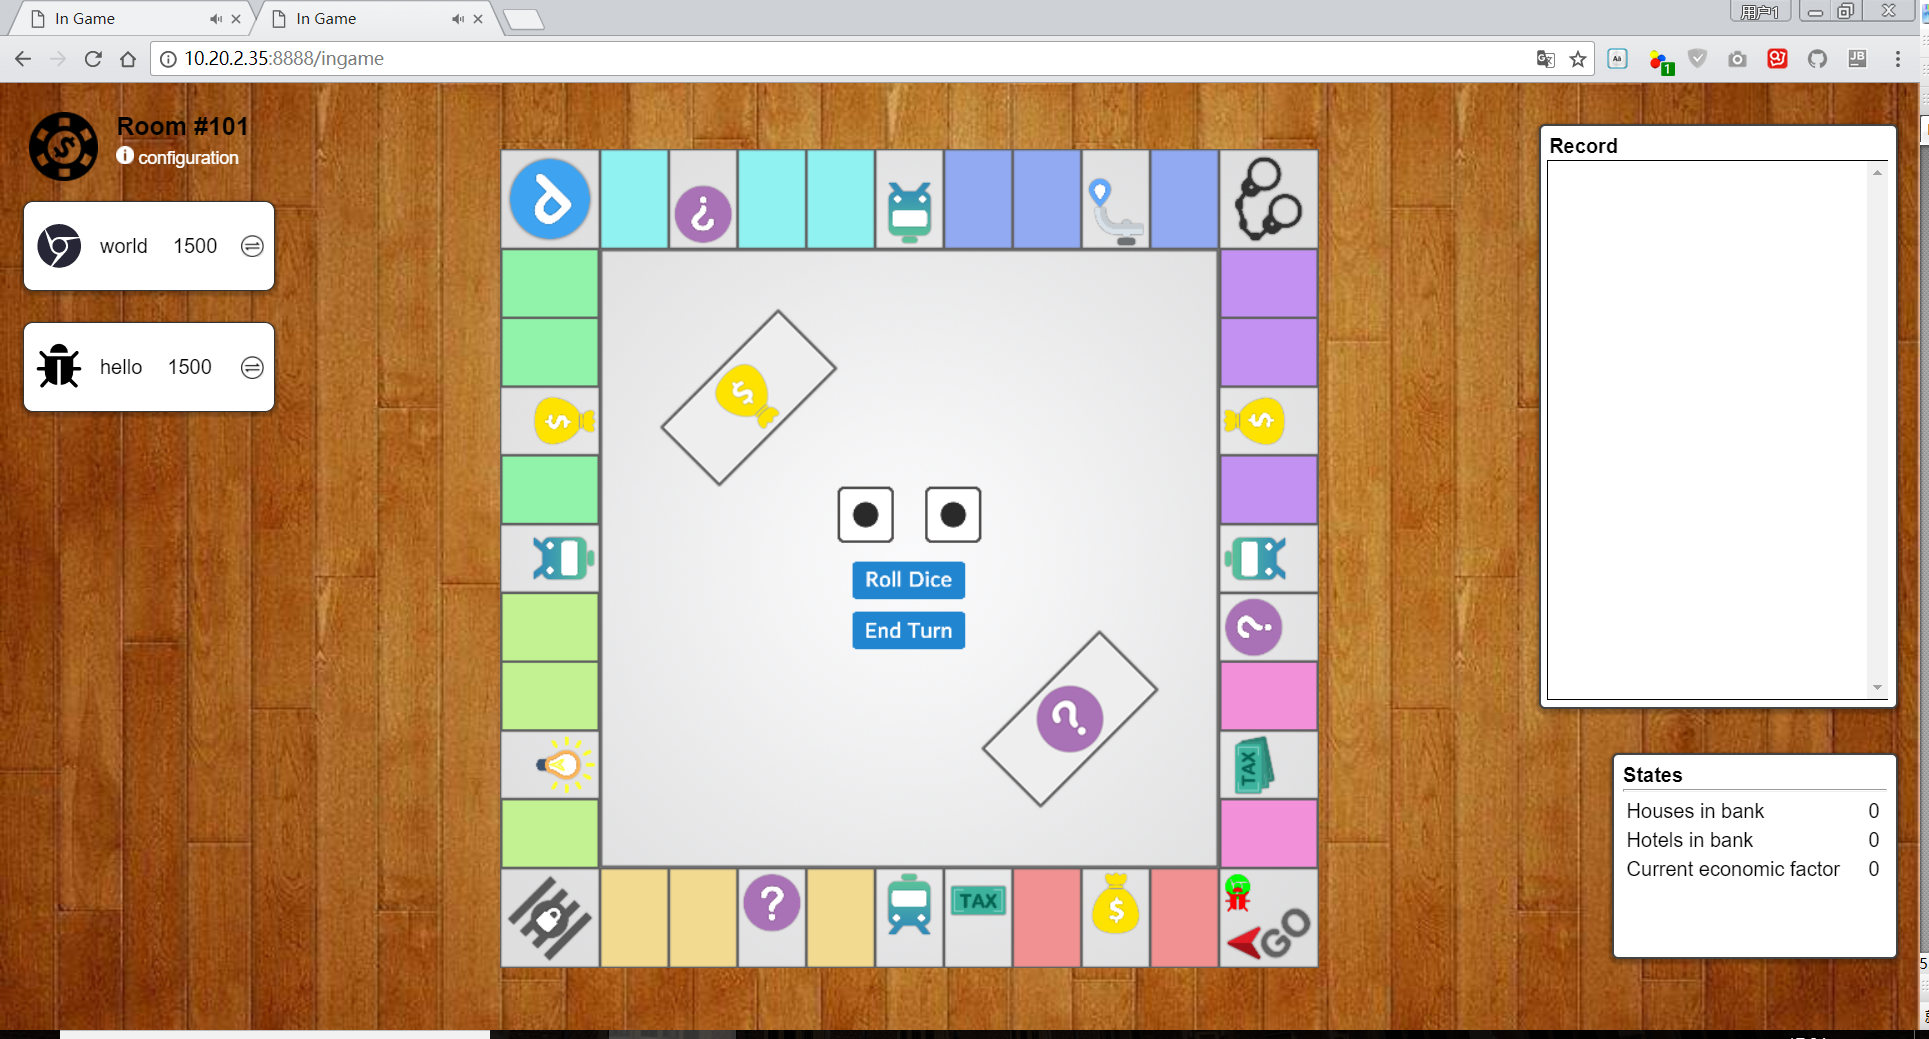
\includegraphics[scale=0.32]{image/ingame1.png}
\caption{Main page 1}
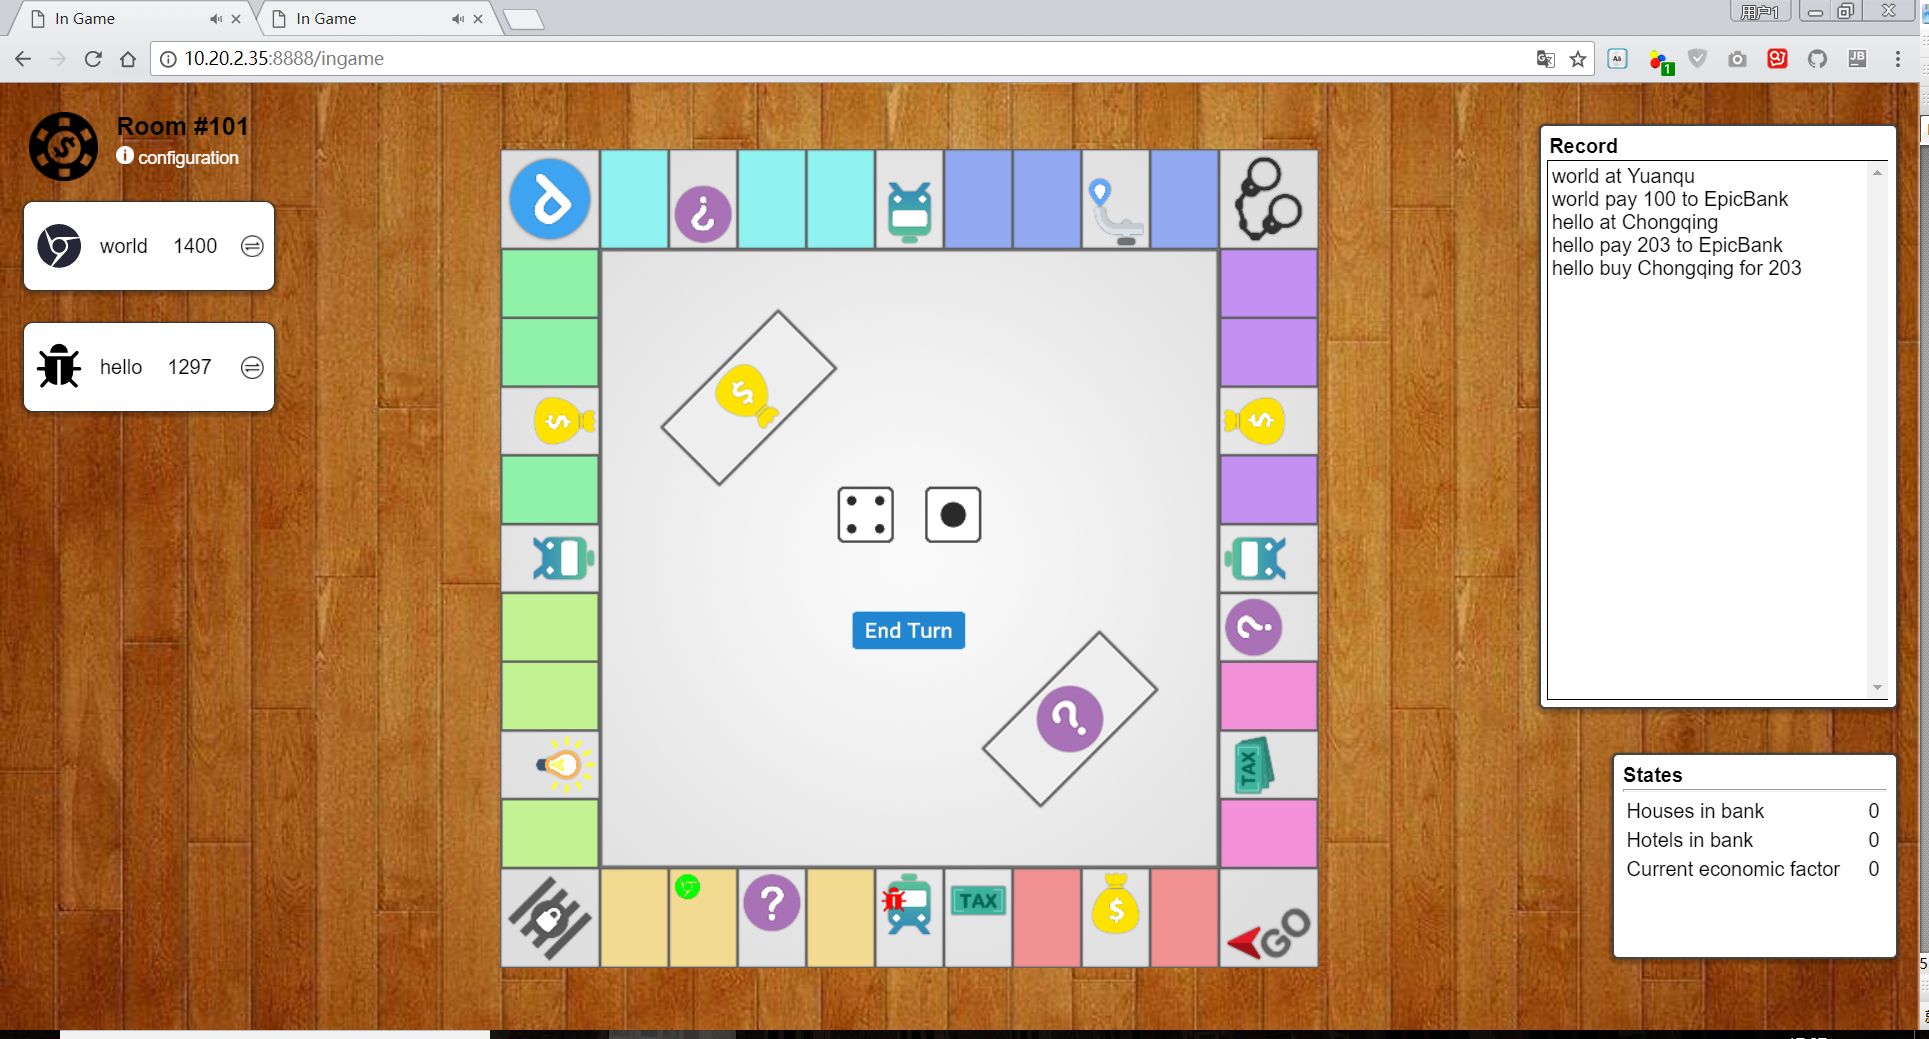
\includegraphics[scale=0.32]{image/ingame3.png}
\caption{Main page 2}
\end{figure}
\begin{figure}[htbp]
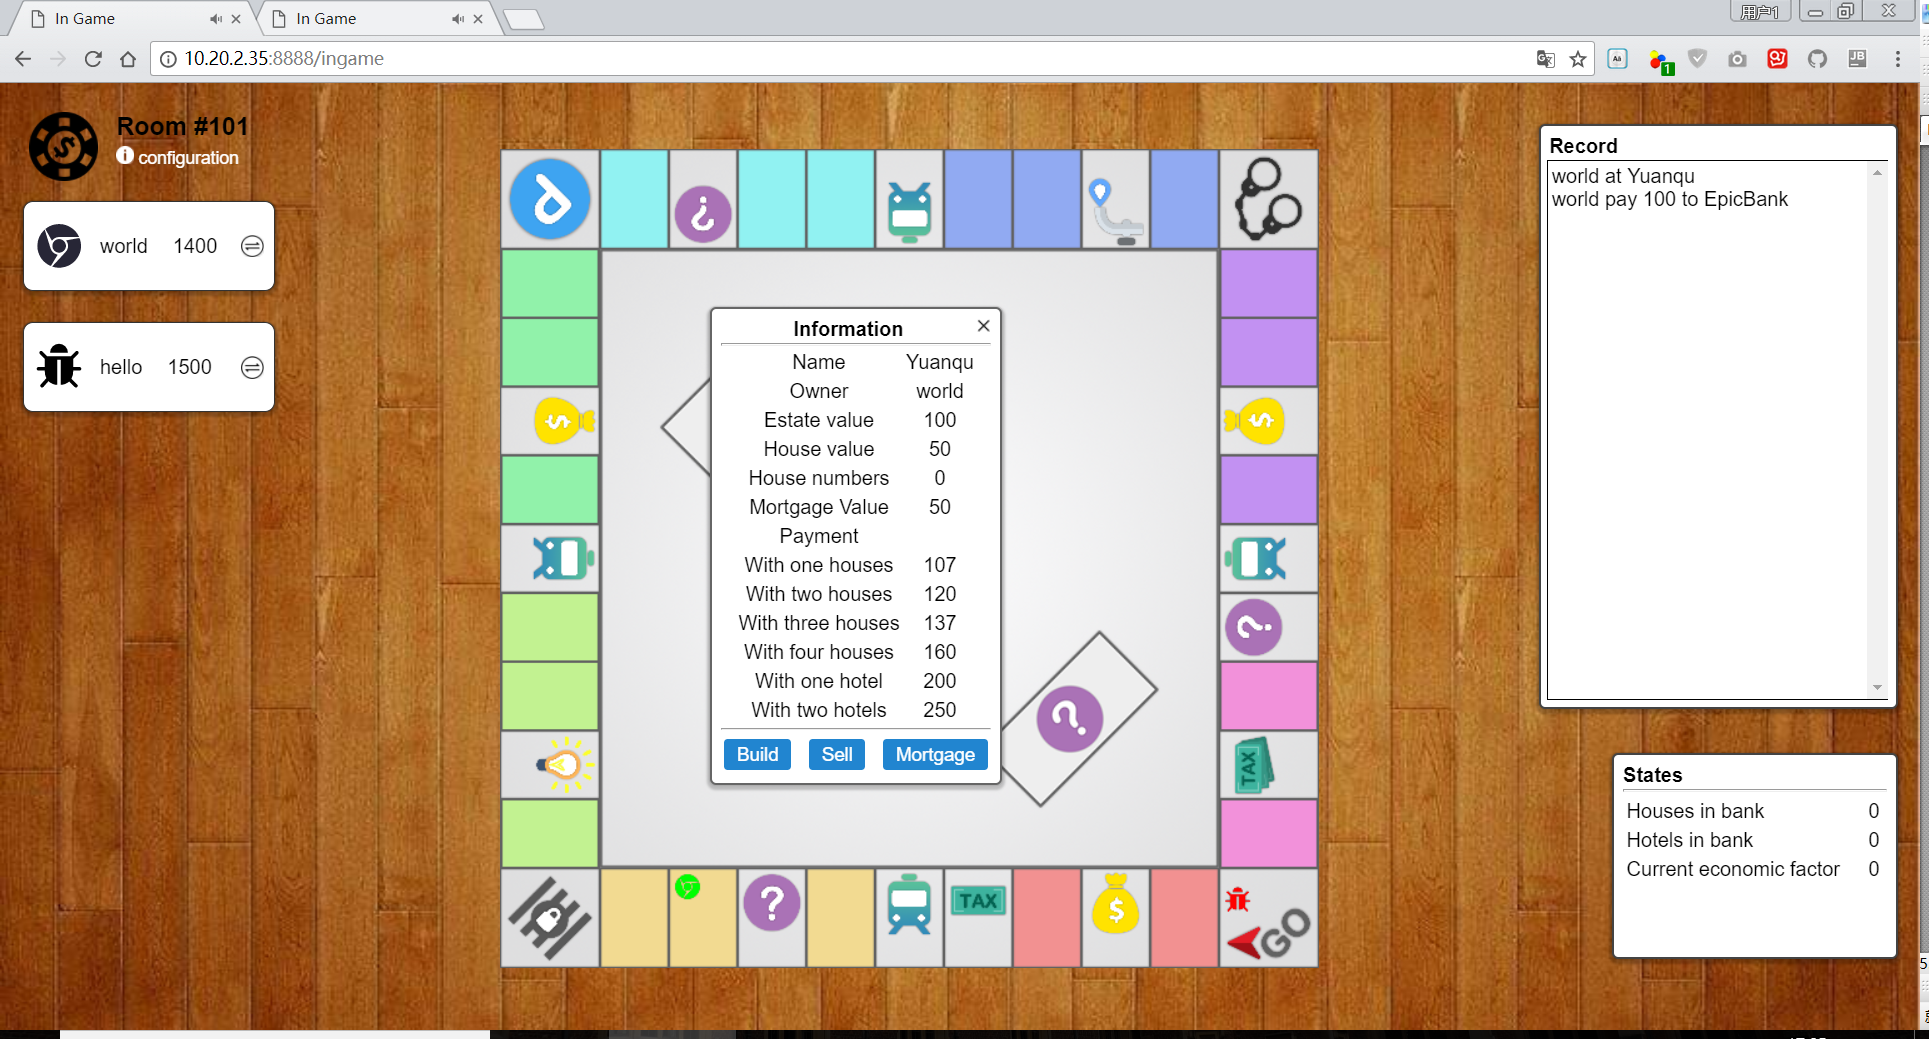
\includegraphics[scale=0.32]{image/ingame2.png}
\caption{Management page}
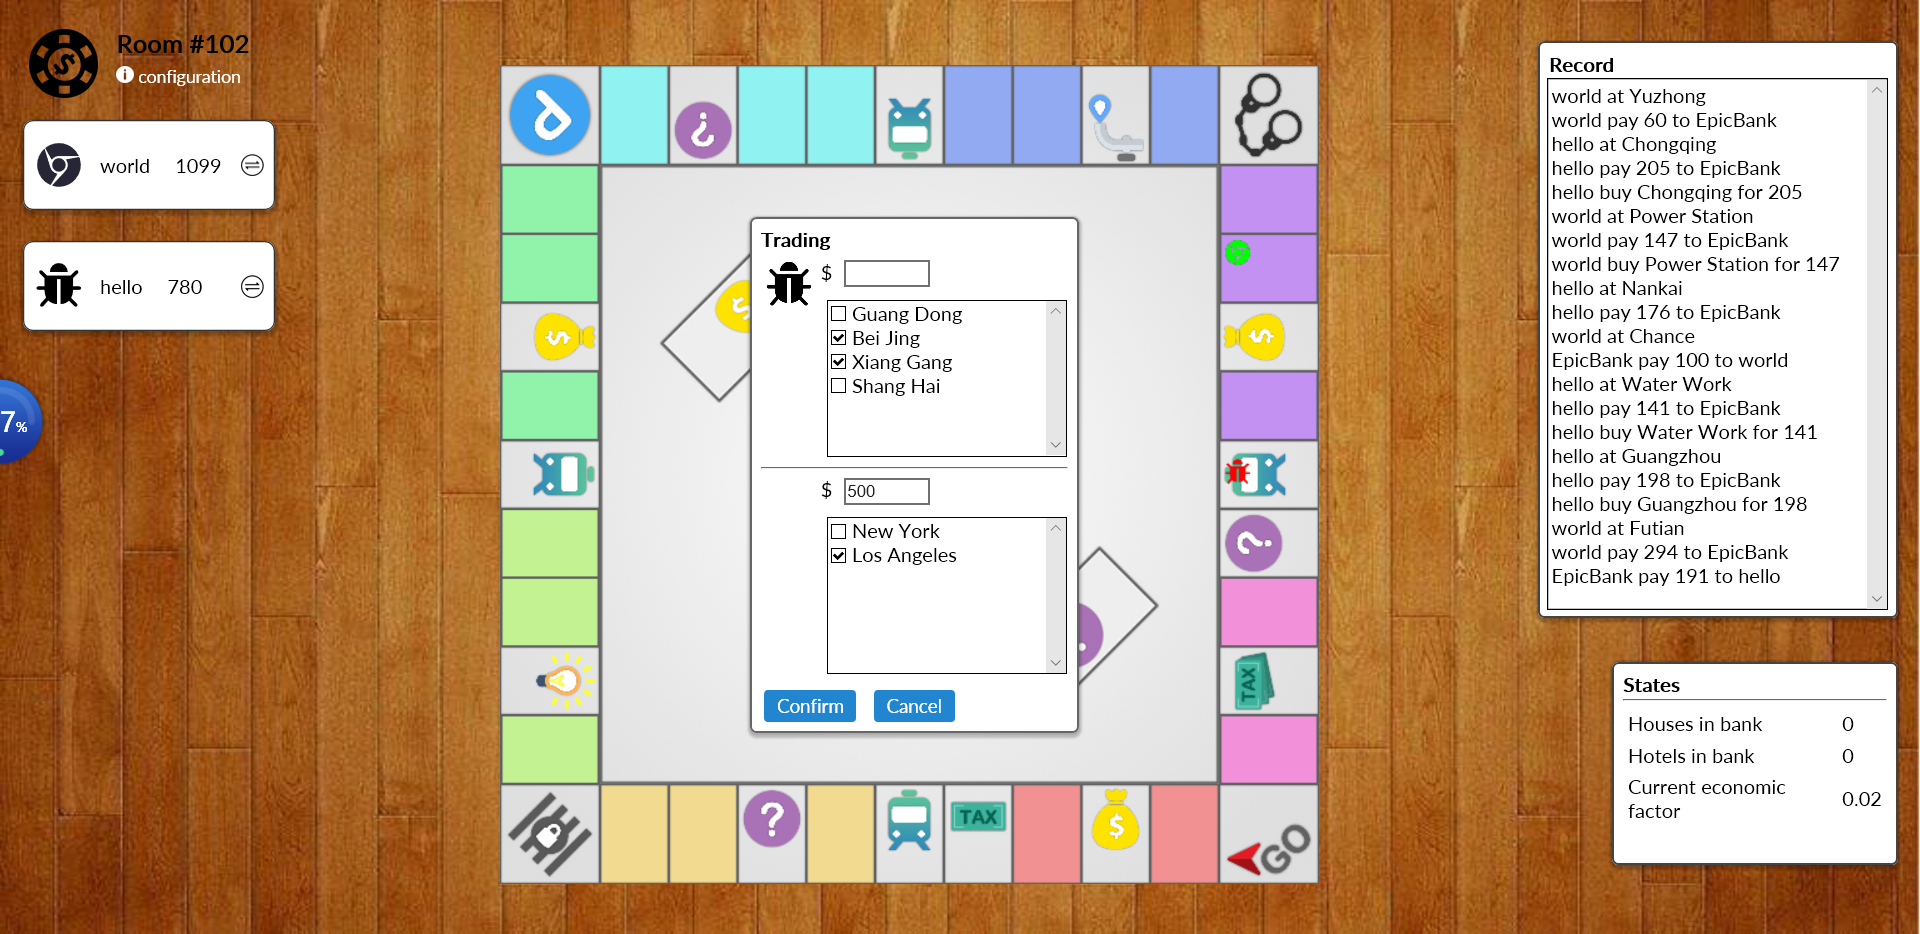
\includegraphics[scale=0.19]{image/trade.png}
\caption{Trade page}
\end{figure}

\end{document}
